\documentclass{beamer}

\usepackage{amsmath,amsthm,enumerate,amssymb,times}
\usepackage{graphicx}
\graphicspath{ {./figures/} }
\usepackage{float, subcaption, wrapfig}
\usepackage[mathscr]{euscript}
\usepackage{amsthm}%\usepackage[serbian]{babel}

\usepackage{fontspec}
\usepackage{polyglossia}
\setmainlanguage[Script=Cyrillic]{serbian}
\setotherlanguage{english}
\setmainfont{CMU Serif}
\setsansfont{Myriad Pro}% or any other sans serif font

\setlength{\unitlength}{5mm}

\theoremstyle{plain}
\newtheorem{thm}{Теорема}
\newtheorem*{lem}{Лема}
\newtheorem*{cor}{Последица}
\theoremstyle{definition}
\newtheorem*{defn}{Дефиниција}

\setbeamertemplate{theorems}[normal font]

\usetheme{Berlin}

\usefonttheme{serif}
\definecolor{darkred}{rgb}{1,1,1 }
\setbeamercolor{block title}{fg=darkred!70!black}
\setbeamercolor{itemize item}{fg=darkred!70!black}
\setbeamertemplate{items}[circle]
%\setbeamercovered{transparent}

\title[Примена теорије група]{Примена теорије група}
\author[Даниел Силађи ]{Даниел Силађи}
\date[мај 2014.]{мај 2014.}
\institute[Гимназија Јован Јовановић Змај]{Гимназија Јован Јовановић Zmaj}

%
%==============================================================================================
%

\begin{document}

\section{Теоријa група}
%================================================================================================
\begin{frame}
\titlepage
\end{frame}
%================================================================================================

%---------------------------------------------------
\begin{frame}
\frametitle{Мотивација}
\begin{itemize}
\item У свакодневном животу срећемо "симетричне" објекте
\item Шта је заправо симетрија?
\item Нешто "изгледа исто" кад га гледамо са различитих страна
\item Формалније: симетрија неког објекта је нека трансформација у простору која пресликава тај објекат у самог себе
\end{itemize}
\centering
\vspace{-0.7cm}

\includegraphics[height=5cm]{sneg}
\end{frame}

\begin{frame}
\frametitle{Мотивација 2}
Људи су приметили да такве трансформације имају нека својства заједничка за све њих:
\begin{itemize}
\item Трансформације су бијективне, за сваку трансофмацију постоји њиј инверзна трансформација која "поништава" њен ефекат.
\item Комбиновањем (композицијом) две трансформације добијамо опет трансформацију
\item Сваки објекат има једну тривијалну симетрију, идентичко пресликавање - свака тачка се слика у саму себе
\end{itemize}
\end{frame}

\begin{frame}
\frametitle{Пример - симетрије многоуглова}
\begin{columns}[T]
    \begin{column}{0.5\textwidth}
      \centering
      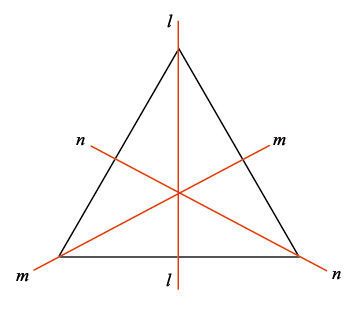
\includegraphics[width=\textwidth]{trougao}
    \end{column}
    \begin{column}{0.5\textwidth}
      \begin{itemize}
         \item Ротације око центра троугла: $r$ (за $\pi/3$), $r\circ r = r^2$ (за $2\pi/3$) и $r\circ r \circ r = r^3 = e$ (за $2\pi$, односно $0$ радијана - идентичко пресликавање)
         \item Осне симетрије $s_1$, $s_2$ и $s_3$ у односу на праве $l$, $m$, $n$.
         \item Слично, важи $s_i \circ s_i = s_i^2 = e$, за $i\in \lbrace 1, 2, 3 \rbrace$, али и $s_1 s_2 = r^2$, ...
       \end{itemize}
    \end{column}
  \end{columns}
\end{frame}

\begin{frame}
\frametitle{Пример - frieze и wallpaper цртежи}
\begin{columns}[T]
    \begin{column}{0.5\textwidth}
      \centering
      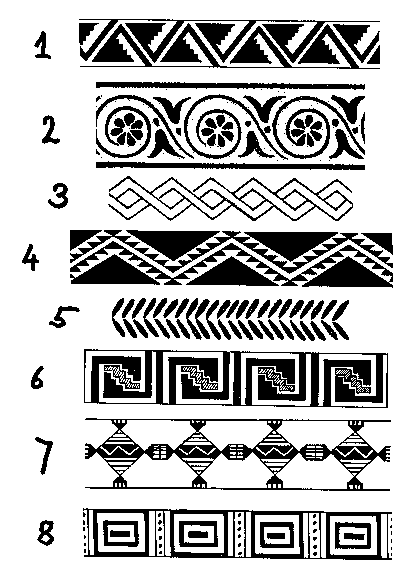
\includegraphics[height=\textwidth]{frieze}
    \end{column}
    \begin{column}{0.5\textwidth}
      \centering
      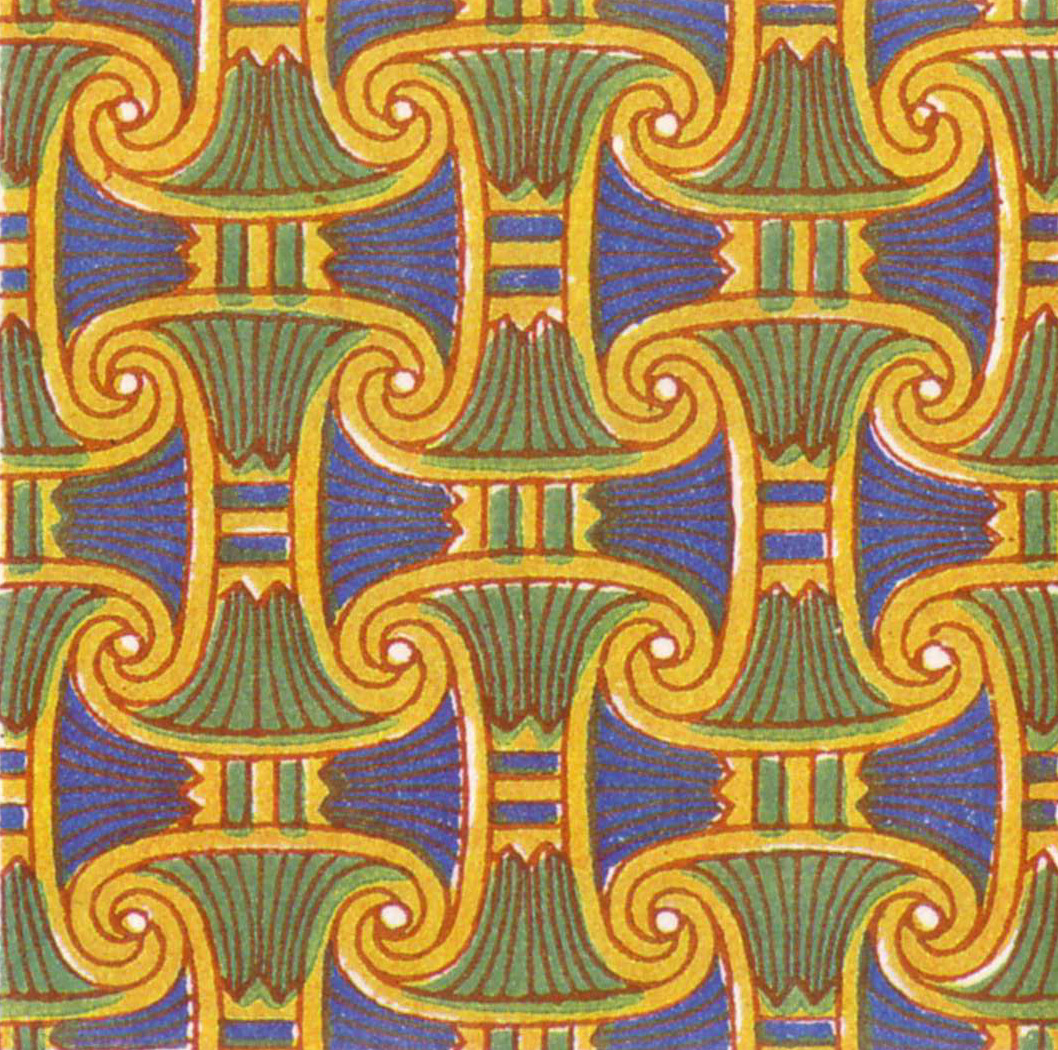
\includegraphics[width=\textwidth]{wallpaper}
    \end{column}
\end{columns}
\end{frame}

\begin{frame}
\frametitle{Пример - молекулске и кристалне симетрије}
\begin{columns}[T]
    \begin{column}{0.5\textwidth}
      \centering
      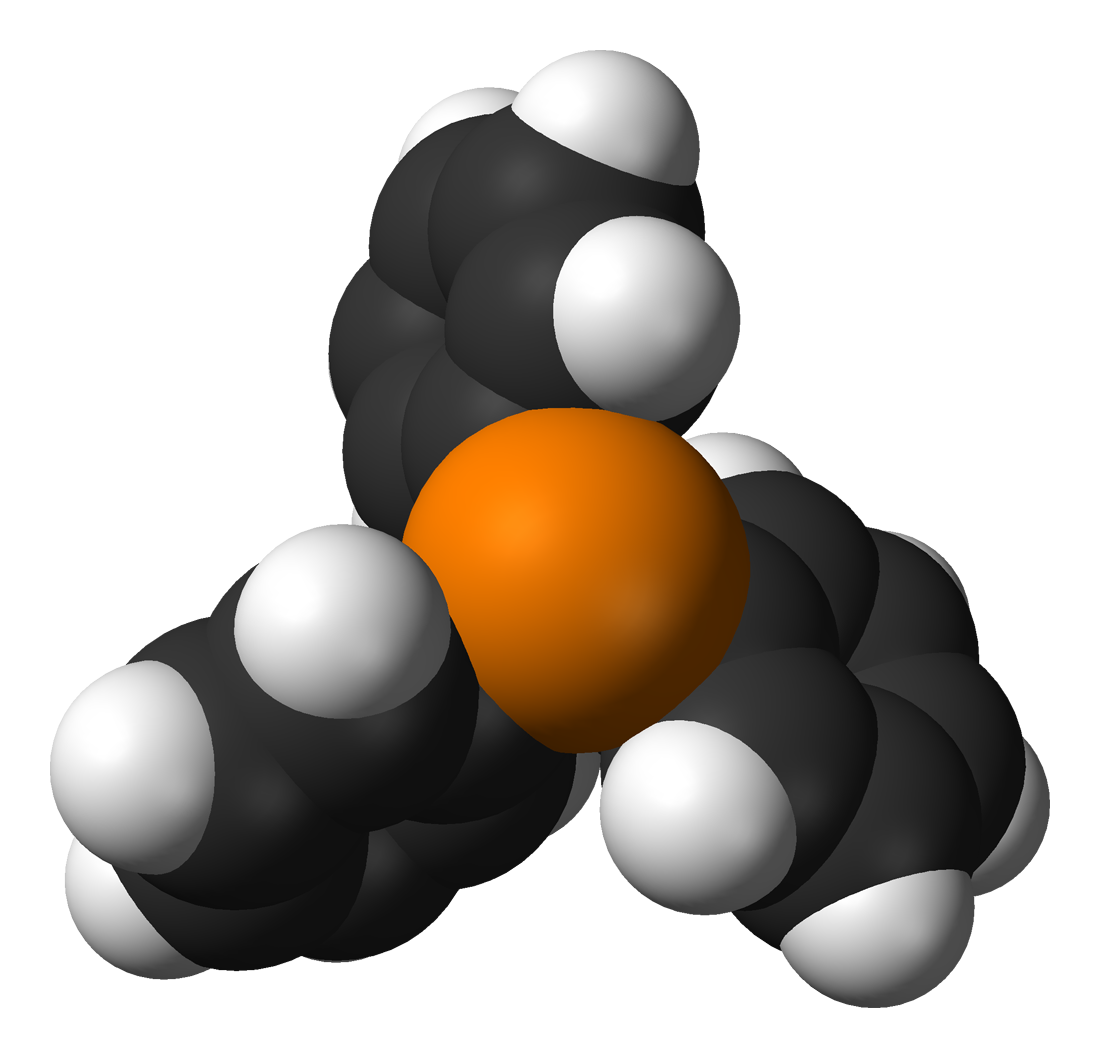
\includegraphics[width=\textwidth]{molekul1}
    \end{column}
    \begin{column}{0.5\textwidth}
      \centering
      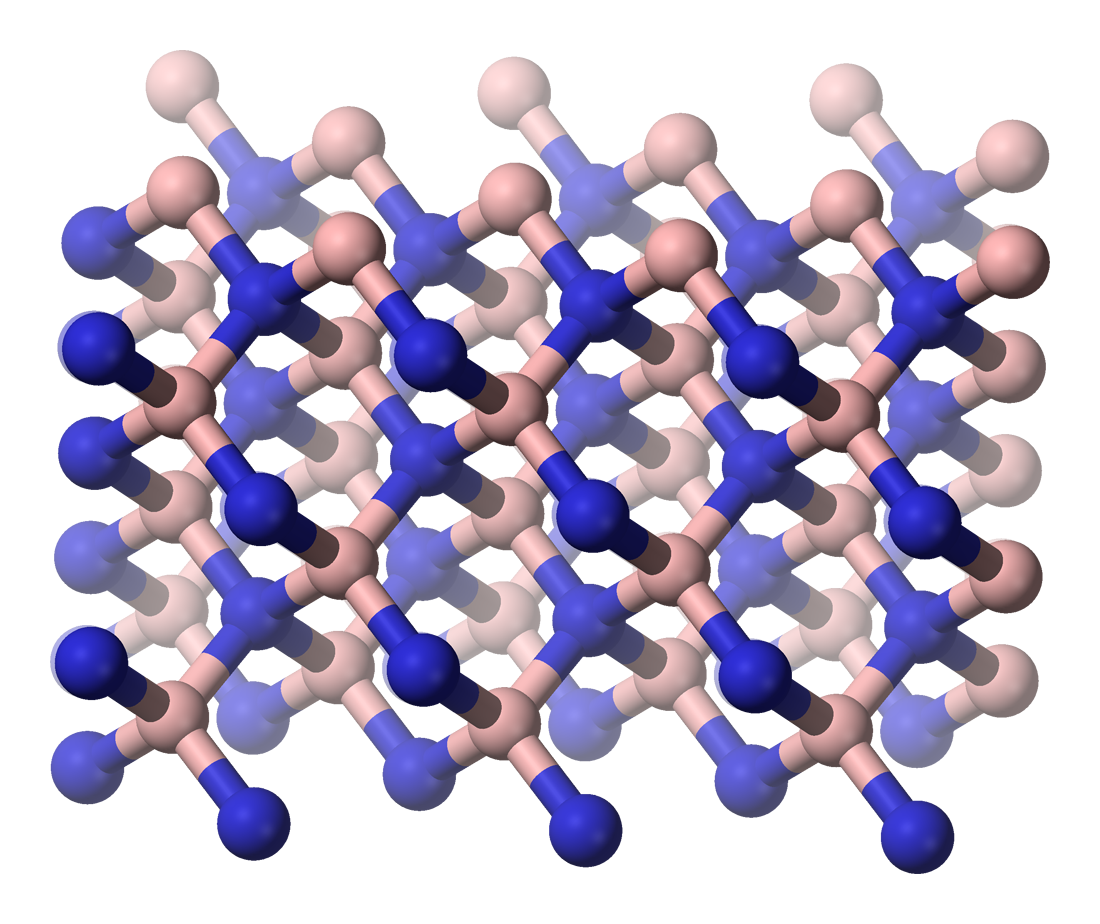
\includegraphics[width=\textwidth]{resetka}
    \end{column}
\end{columns}
\end{frame}

\begin{frame}
\frametitle{Основне дефиниције}
Елементи неке групе не морају нужно да буду трансформације, већ елементи произвољног скупа $G$, за које смо дефинисали операцију "множења", са следећим особинама:
\begin{enumerate}
  \item Ако $a$ и $b$ припадају $G$, онда и њихов производ, $ab$ припада $G$
  \item Операција множења је асоцијативна, односно важи $a(bc) = (ab)c$
  \item $G$ садржи \emph{јединични елемент} $e$, за који важи $ae = ea = a$, за свако $a\in G$
  \item За свако $a\in G$ постоји $b\in G$, за које важи $ab = ba = e$. Такав $b$ се зове \emph{инверзни елемент} за $a$, и обележава се са $a^{-1}$
\end{enumerate}
\end{frame}

\begin{frame}
\frametitle{Примери група}
Иако операцију групе често називамо ''множењем'', она заправо и може а и не мора то да буде:
\begin{itemize}
  \item Скуп рационалних (или реалних) бројева без $0$ чини групу у односу на множење (у уобичајеном смислу)
  \item Скуп целих (али не и природних!) бројева чини групу у односу на сабирање
  \item Скуп свих инвертибилних (регуларних, њихова детерминанта је различита од $0$) квадратних матрица, над пољем $\mathbb{R}$ или $\mathbb{C}$, димензија $n\times n$, чини групу, а операција групе је множење матрица.
\end{itemize}
\end{frame}

\begin{frame}
\frametitle{Неке корисне ознаке и дефиниције}
\begin{itemize}
  \item Ако је операција групе комутативна, група је комутативна или \emph{Абелова}
  \item $a^n \equiv \underbrace{aa...a}_{n\text{ пута}} $, и $a^{-n} \equiv (a^{-1})^n = (a^n)^{-1}$
  \item Ако су сви степени $a$ различити, група је \emph{бесконачног реда}. Иначе, \emph{ред елемента} је најмање $n\in \mathbb{N}$ за које важи $a^n = e$
  \item \emph{Ред групе} је број елементата те групе
  \item Непразан подскуп $H$ групе $G$ је \emph{подгрупа} групе $G$, ако је $H$ група у односу на рестрикцију операције групе $G$ на $H$
  \item $\langle A\rangle$ је \emph{подгрупа генерисана скупом $A$} - најмања подгрупа $G$ која садржи скуп $A$. Ако је $\langle A\rangle=G$, онда је $A$ \emph{генераторни скуп} групе $G$, а његови елементи - \emph{генератори} групе $G$.
\end{itemize}
\end{frame}

\begin{frame}
\frametitle{Пермутације}
\begin{itemize}
  \item \emph{Пермутације} скупа $\{1, 2, ..., n\}$ су све функције $\pi$ које бијективно пресликавају тај скуп у самог себе
  \item Записују се као $$\pi = \begin{pmatrix}
            1 & 2 & ... & n \\
            a_1 & a_2 & ... & a_n
        \end{pmatrix},$$
 где важи $\{a_1, a_2, ..., a_n\} = \{1, 2, ..., n\}$, и $\pi(i) = a_i$, за $1\leq i\leq n$
  \item Пермутације $n$ елемената чине групу $S_n$, \emph{симетричну групу}
  \item Кејлијева (Cayley) теорема: Свака група $G$ реда $n$ је изоморфна са подгрупом симетричне групе $S_n$.
\end{itemize}
\end{frame}

\begin{frame}
\frametitle{Лагранжова теорема}
\begin{thm}
Ако је $G$ нека група реда $n$, и $H$ њена подгрупа реда $m$, тада $m$ дели $n$.
\end{thm}
\begin{itemize}
\item У доказу, поделили смо групу $G$ на $k$ дисјунктних подскупова:
$$G = H \cup a_1 H \cup a_2 H \cup ... \cup a_{k-1} H$$
\item Број $k$ се зове \emph{индекс} подгрупе $H$ у групи $G$
\item Скупови $a_i H$ се зову \emph{леве класе} $H$ у $G$
\item Скуп свих левих класа неке подгрупе се обележава са $G/H$
\end{itemize}
\end{frame}

\begin{frame}
\frametitle{Инваријантне подгрупе}
\begin{itemize}
\item За елемент $b$ групе $G$ кажемо да је \emph{конјугован} елементу $a$ ако постоји $u\in G$ за који важи
$$u a u^{-1} = b$$
\item Релација конјугације је релација еквиваленције, разбија групу на класе конјугације
\item Посматрајмо подгрупу $H$ групе $G$. Тада се лако показује да је и $aHa^{-1}$ (сви производи $aha^{-1}$, где $h\in H$) подгрупа од $G$, при чему је $a$ произвољни елемент из $G$. Уколико за свако $a\in G$ важи
$$aHa^{-1} = H,$$
тада кажемо да је $H$ \emph{инваријантна} или \emph{нормална подгрупа} групе $G$, и то обележавамо са $H\lhd G$.
\end{itemize}
\end{frame}

\begin{frame}
\frametitle{Инваријантне подгрупе - наставак}
\begin{itemize}
\item За неку групу $G$ и њену нормалну подгрупу $H$ дефинишимо операцију $\cdot: G/H \to G/H$ као $aH\cdot bH := abH$
\item Скуп свих левих класа $G/H$ (у случају да је $H\lhd G$) група у односу на овако дефинисану операцију
\item Јединични елемент је $eH = H$, а инверзни елемент за класу $aH$ је $a^{-1}H$
\item Овако добијена група се назива \emph{фактор-група}, обележава се са $G/H$
\item Њен ред индекс групе $H$ у $G$
\item Пример: $\mathbb{Z}/n\mathbb{Z}$, и сабирање
\end{itemize}
\end{frame}

\section{Векторски простори}

\begin{frame}
\frametitle{Векторски простори}
Нека је $(V, +)$ комутативна група, а $(F, +, \cdot)$ поље. $V$ је \emph{векторски простор над пољем} $F$, ако је дефинисано пресликавање $F\times V\to V$, при чему слику пара $(\alpha, v)$ означавамо са $\alpha v$, тако да за свако $\alpha, \beta \in F$, $u, v\in V$ важи:
\begin{enumerate}
\item $\alpha(u+v) = \alpha u+\alpha v$
\item $(\alpha + \beta)v = \alpha v+ \beta v$
\item $(\alpha\cdot\beta)v = \alpha(\beta v)$
\item $1v = v$
\end{enumerate}
где је са $1$ означен неутрални елеменат за множење поља $F$. Елементи скупа $F$ се називају \emph{скалари}, а елементи скупа $V$ - \emph{вектори}. Ми ћемо у овом раду посматрати искључиво поља реалних и комплексних бројева.
\end{frame}

\begin{frame}
\frametitle{База векторског простора}
\begin{itemize}
\item \emph{База} векторског простора је низ вектора који је линеарно независан и који генерише векторски простор.
\item Још алтернативних дефиниција:
\begin{itemize}
  \item Низ вектора је база ако и само ако је тај скуп максималан линеарно независан скуп.
  \item Низ вектора је база ако и само ако је тај скуп минималан скуп генератора
  \item Низ вектора $v_1, ..., v_n$ је база ако и само ако се сваки вектор $x\in V$ може на јединствен нaчин написати у облику $$x = \sum_1^n\alpha_i v_i, \quad \alpha_1, ..., \alpha_n\in F$$
\end{itemize}
\item Све базе неког одређеног векторског простора $V$ имају исти број елемената - \emph{димензија векторског простора}, $\operatorname{dim} V$
\end{itemize}
\end{frame}

\begin{frame}
\frametitle{Унитарни векторски простор}
Нека је $V$ векторски простор над пољем $F$ (где је $F=\mathbb{R}$ или $F=\mathbb{C}$). \emph{Унутрашњи (скаларни) производ} на $V$ је свака функција $(,):V\times V\to F$, при чему слику уређеног пара вектора $(x, y)\in V\times V$ означавамо са $(x, y)$, за коју за свако $x, y, z\in V$ и свако $\alpha \in F$ важи
\begin{enumerate}
  \item $(x, y) = \overline{(y, x)}$
  \item $(x+y, z) = (x, z)+(y, z)$
  \item $(\alpha x, y) = \alpha (x, y)$
  \item $(x, x)\geq 0$
  \item $(x, x) = 0 \Leftrightarrow x=0$
\end{enumerate}
\end{frame}

\begin{frame}
\begin{itemize}
\item У унитарном векторском простору $V$ функција $\|\;\|:V\to \mathbb{R}$, дефинисана са $$\|x\| = \sqrt{(x, x)}$$ назива се \emph{норма} на $V$
\item Ненегативан реалан број $\|x\|$ назива се \emph{норма вектора} $x$
\item \emph{Растојање} вектора $x$ и $y$ је дефинисано са $$d(x, y) = \|x-y\|.$$
\item У унитарном векторском простору $V$ за свако $x, y\in V$ важи
$$|(x, y)|\leq\|x\|\|y\|,$$
при чему једнакост важи ако и само ако су вектори $x$ и $y$ линеарно зависни.
\end{itemize}

\end{frame}

\begin{frame}
\begin{itemize}
\item У еуклидским векторским просторима можемо дефинисати угао између вектора $x\neq 0$ и $y\neq 0$, као реалан број $\alpha\in [0, \pi]$, такав да је $$\cos \alpha = \frac{(x, y)}{\|x\|\|y\|}$$
\item За два вектора $x$ и $y$ кажемо да су \emph{ортогонални} ако је $(x, y) = 0$.

\item За базу $B=\{b_1, ..., b_n\}$ неког унитарног векторског простора $V$ кажемо да је \emph{ортонормирана}, ако је
$$(b_i, b_j) = \begin{cases}
                1 & \mbox{ако } i=j \\
                0 & \mbox{ако } i\neq j
               \end{cases}$$
\item Сваки унитарни векторски простор поседује бар једну ортонормирану базу, и она се може добити из произвољне базе применом \emph{Грам-Шмитовог поступка}
\end{itemize}
\end{frame}

\section{Линеарне трансформације}

\begin{frame}
\frametitle{Линеарне трансформације}
\begin{defn}
Нека су $V_1$ и $V_2$ векторски простори над истим пољем $F$. Пресликавање $A: V_1\to V_2$ такво да је
$$(\forall a, b\in V_1)(\forall \alpha, \beta \in F) A(\alpha a+ \beta b) = \alpha A(a) + \beta A(b)$$
назива се \emph{линеарна трансформација (линеарни оператор, хомоморфизам)} векторског простора $V_1$ у $V_2$. Уколико је $V_1 = V_2 = V$, тада је $A$ просто линеарна трансформација векторског простора $V$.
\end{defn}
\end{frame}

\begin{frame}
\frametitle{Матрица линеарне трансформације}
\begin{itemize}
\item Претпоставимо да је $\{a_1, ...a_n\}$ база векторског простора $V$. Тада, линеарну трансформацију $A$ можемо задати са
$$A(a_1) = b_1, A(a_2) = b_2, ..., A(a_n) = b_n$$
где су $b_1, ..., b_n\in V$.
\item Пошто је $\{a_1, ...a_n\}$ база, сваки од вектора $b_i$ може се на јединствен начин написати као линеарна комбинација вектора базе, па имамо:
$$A(a_1) = \alpha_{11}a_1 + \alpha_{21}a_2 + ... + \alpha_{n1}a_n$$
$$A(a_2) = \alpha_{12}a_1 + \alpha_{22}a_2 + ... + \alpha_{n2}a_n$$
$$...$$
$$A(a_n) = \alpha_{1n}a_1 + \alpha_{2n}a_2 + ... + \alpha_{nn}a_n$$
\end{itemize}
\end{frame}

\begin{frame}
\begin{itemize}
\item Ако напишемо коефицијенте $\alpha_{ij}$ као матрицу, вредност функције $A(x)$ (као линеарне трансформације произвољног вектора $x\in V$) можемо израчунати простим множењем матрица:
$$[A(x)] = [A][x] = \begin{bmatrix}
            \alpha_{11} & \alpha_{12} & ... & \alpha_{1n} \\
            \alpha_{21} & \alpha_{22} & ... & \alpha_{2n} \\
            ... & ... & ... & ... \\
            \alpha_{n1} & \alpha_{n2} & ... & \alpha_{nn}
           \end{bmatrix}
           \begin{bmatrix}
           \zeta_1\\
           \zeta_2\\
           \vdots \\
           \zeta_n
           \end{bmatrix}
$$
при чему је $x = \zeta_1 a_1 + \zeta_2 a_2 + ... \zeta_n a_n$.
\item Матрични запис линеарне трансформације зависи од избора базе!
\end{itemize}
\end{frame}

\section{Групе у физици}
\begin{frame}
\frametitle{Групе матрица}
\begin{itemize}
\item \emph{Општа линеарна група, $GL(n, \mathbb{C})$} скуп свих $n\times n$ регуларних (инвертибилних, детерминанта различита од 0) матрица над $\mathbb{C}$, у односу на множење матрица. Ове матрице одговарају свим инвертибилним линеарним трансформацијама простора $\mathbb{C}^n$. Њена подгрупа је $GL(n, \mathbb{R})$, скуп свих инвертибилних реалних матрица $n\times n$ у односу на множење.
  \item \emph{Специјална линеарна група}, $$SL(n, \mathbb{C}) = \{M\in GL(n, \mathbb{C})|\det M = 1\}.$$ Слично,
  $$SL(n, \mathbb{R}) = \{M\in GL(n, \mathbb{R})|\det M = 1\}.$$
\end{itemize}
\end{frame}

\begin{frame}
\begin{itemize}
\item \emph{Унитарна група, $U(n)$}
  $$U(n) = \{M\in GL(n, \mathbb{C})|MM^\dag = I\}.$$
  Чува скаларни производ вектора $x = (x_1, ..., x_n)$, $y = (y_1, ...y_n)$:
  $(Mx, My) = (x, y) = \sum_{i=1}^n x_i \overline{y}_i.$
\item \emph{Специјална унитарна група}: $SU(n) = \{M\in U(n)|\det M = 1\}.$
\item \emph{Ортогонална група}: $O(n) = \{M\in GL(n, \mathbb{R})|MM^T = 1\}.$
  Слично као унитарна група, чува стандардни скаларни производ
  $(Mx, My) = (x, y) = \sum_{i=1}^n x_i y_i.$
\item \emph{Специјална ортогонална} група, $SO(n) = \{M\in O(n)|\det M = 1\}.$
\end{itemize}
\end{frame}

\begin{frame}
\frametitle{Псеудоортогонална група}
\begin{itemize}
\item Нека је $g$ дијагонална матрица $g = \operatorname{diag}(\underbrace{1, .., 1}_p, \underbrace{-1, ..., -1}_q)$.
\item Псеудоортогонална група $O(p, q)$ се дефинише као
      $$O(p, q) = \{M\in GL(n, \mathbb{R})|M^TgM = g\}.$$
\item То управо матрице које чувају квадратну форму
      $$\sum_{i=1}^p x_iy_i - \sum_{i=1}^q x_{p+i}y_{p+i}.$$
\item Најпознатија група ове врсте је Лоренцова група $O(1, 3)$, са којом ћемо се позабавити на крају овог рада.
\end{itemize}
\end{frame}

\begin{frame}
\frametitle{Симетрије унитарних векторских простора}
\begin{defn}
Нека је дат еуклидски векторски простор $V$ коначне димензије.
\begin{description}
  \item[Изометријске трансформације] су трансформације (пресликавања) $M: V\to V$, које чувају растојање, тј. за свако $u,v\in V$ важи
  $$\|u-v\| = \|M(u)-M(v)\|$$
  \item[Ортогоналне трансформације] су трансформације $M: V\to V$ које чувају скаларни производ, тј. за све $u, v, \in V$
  $$(u, v) = (M(u), M(v))$$
\end{description}
\end{defn}
\end{frame}

\begin{frame}
\frametitle{Две теореме}
\begin{thm}
Нека је $M:V\to V$ ортогонално пресликавање еуклидског векторског простора. Тада је $M$ изометријска трансформација која чува 0, тј. $M(0) = 0$.
\end{thm}
\begin{thm}
Нека је $M$ изометрија неког еуклидског векторског простора и нека је $M(0) = 0$. Тада је $M$ ортогонална трансформација
\end{thm}
\end{frame}

\begin{frame}
\frametitle{...и трећа теорема}
\begin{thm}
Ако је $M$ ортогонална трансформација коначнодимензионалног еуклидског простора, тада важи
\begin{enumerate}
  \item $M$ је линеарна трансформација
  \item Ако је $[M]$ матрица трансформације $M$ у односу на неку ортонормирану базу, тада важи $[M]^T[M] = I$
  \item $M$ је инвертибилна и $M^{-1}$ је такође изометрија
  \item $\det [M]=\pm 1$ (у било којој бази)
\end{enumerate}
\end{thm}
\end{frame}

\section{Лоренцова група}

\begin{frame}
\frametitle{Лоренцове трансформације и метрика Минковског}
\begin{itemize}
\item У специјалној теорији релативности, једина инваријантна метрика у простор-времену је \emph{метрикa Минковског}:
$$\Delta s^2 = c^2\Delta t^2 - \Delta x^2 - \Delta y^2 - \Delta z^2$$
\item Лоренцове трансформације можемо посматрати као "ротације" простор-времена, аналогно ротацијама тродимензионалног еуклидског простора (које чувају метрику $s^2 = x^2+y^2+z^2$)
\item Такође, $s^2 = X\cdot X = X^T\eta X,$
при чему је матрица $\eta$ (понекад и њу називамо метриком Минковског) дата са
$$\begin{bmatrix}
    1 &  0 &  0 &  0\\
    0 & -1 &  0 &  0\\
    0 &  0 & -1 &  0\\
    0 &  0 &  0 & -1
  \end{bmatrix}$$
\end{itemize}
\end{frame}

\begin{frame}
\frametitle{Лоренцовa група}
\begin{itemize}
\item Тражимо решења матричне једначине $\Lambda^T \eta \Lambda = \eta$
\item Очекујемо и добијамо 6 независних решења, подељених у 2 класе: просторне ротације и \emph{Лоренцови потисци}
$$\Lambda = \begin{bmatrix}
    1 & 0 & 0 & 0 \\
    0 &   &   &   \\
    0 &   & R &   \\
    0 &   &   &
  \end{bmatrix} \text{ или }
  \Lambda = \begin{bmatrix}
    \gamma & -\gamma v/c & 0 & 0 \\
    -\gamma v/c & \gamma & 0 & 0 \\
    0 &  0 & 1 & 0  \\
    0 & 0  & 0 & 1
  \end{bmatrix}$$
\item $R$ је матрица ротације у 3 димензије, a $\gamma = \frac{1}{\sqrt{1-\frac{v^2}{c^2}}}$.
\item Ове матрице чине групу, $O(1, 3)$ ($\det\Lambda = \pm 1$). Подгрупе: $SO(1, 3)$ ($\det\Lambda = 1$) и њена подгрупа $SO^+(1, 3)$ ($\Lambda_{11}>0$)
\end{itemize}
\end{frame}

\begin{frame}
\frametitle{Лоренцова група и $SL(2, \mathbb{C})$}
\begin{itemize}
\item Представимо вектор $X = (ct, x, y, z)$ као (Хермитску) матрицу
$$\hat X = \begin{bmatrix}
            ct+z & x-iy \\
            x+iy & ct-z
           \end{bmatrix}$$
\item Све $2\times 2$ Хермитске матрице се могу записати у овом облику
\item Згодно својство $X \cdot X = \det \hat X = c^2 t^2 - x^2 - y^2 - z^2$
\item Испоставља се да је $SO(1, 3)^+\cong SL(2, \mathbb{C})/\mathbb{Z}_2$, односно да се све Лоренцове трансформације могу представити матрицама из $SL(2, \mathbb{C})$, и обрнуто
\item Свели смо један потпуно "физички" проблем на чисту математику!

\end{itemize}
\end{frame}

%========================

\section{}
\begin{frame}
\frametitle{}
\centering
{\Huge Хвала на пажњи!}

\end{frame}
%-------------------------------

\end{document}


